\section{Геометрические свойства модели Изинга с точки зрения числа соседей в узлах}

\subsection{Сравнение модели Изинга и полимерной цепочки в решетках с 2-6 возможными соседями у мономеров}

\begin{figure}
    \centering
    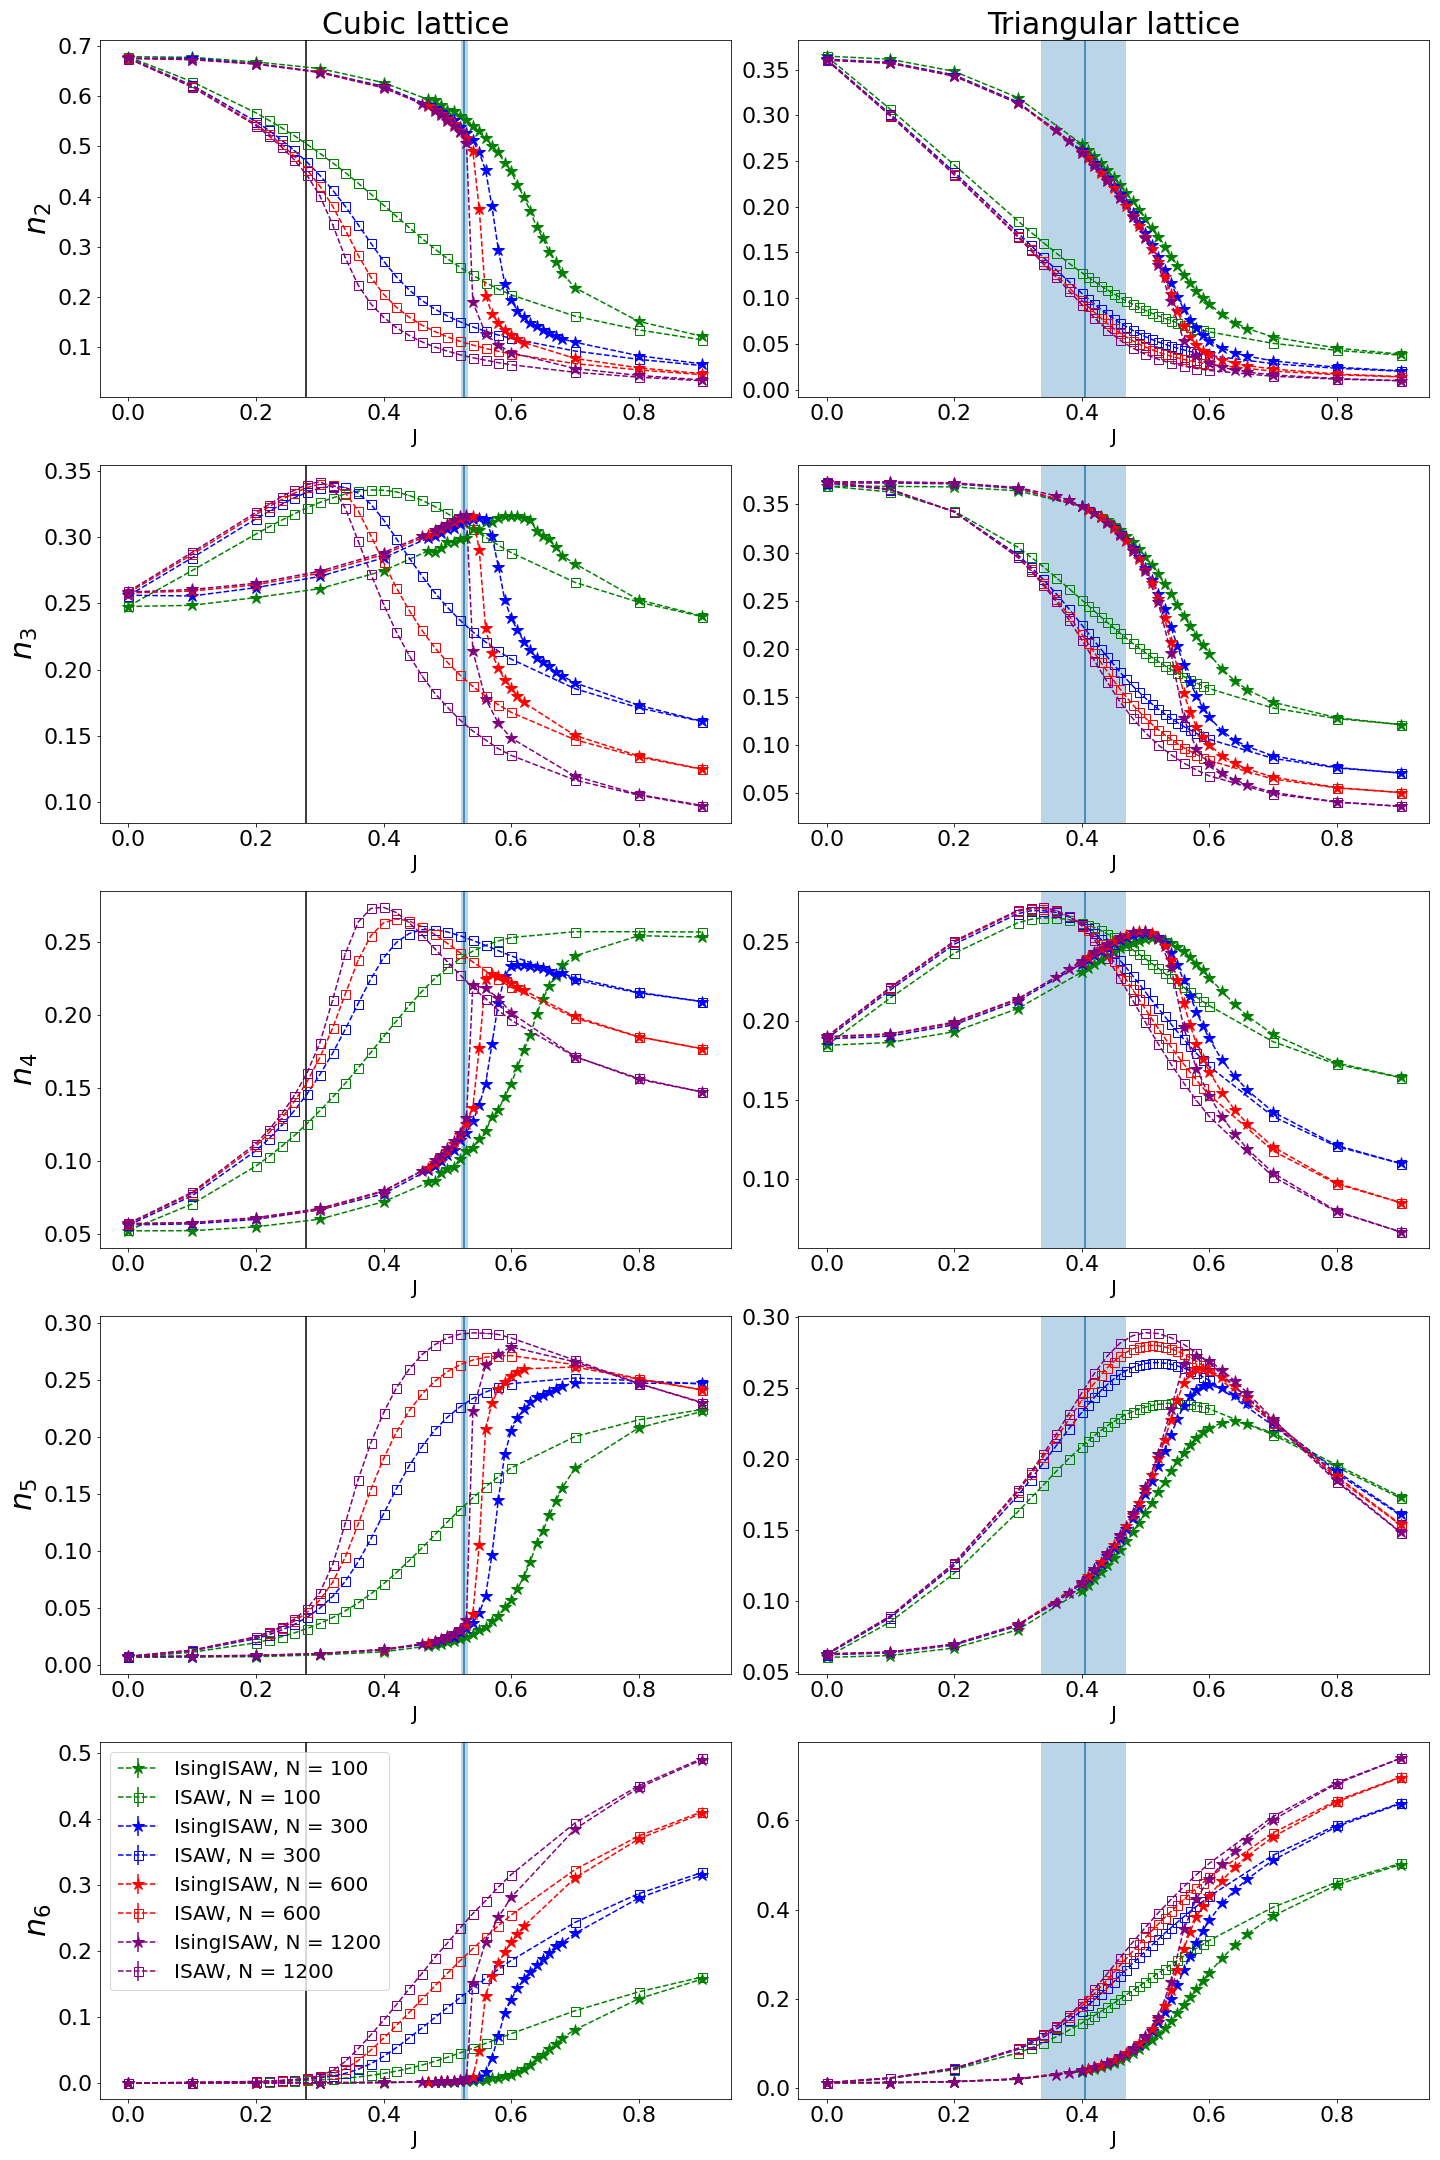
\includegraphics[width=0.95\textwidth, height=21.5cm]{Sections/Images/Ising_vs_ISAW.png}
    \caption{Fractions of monomers of Ising-ISAW model (stars) and ISAW model (open squares) on a cubic lattice (left column) and 2D-triangle lattice (right column) with 2-6 nearest neighbors as function of $J$ with length of conformations $N = $ 100 (green), 300 (blue) and 600 (red). Vertical lines define points of $\theta$-transition (For cubic lattice: black line for ISAW model \cite{Tesi1996} and blue line for Ising-ISAW model \cite{Foster2021}; for triangle lattice: blue line for ISAW model \cite{Privman1986})}
    \label{fig:Ising_vs_ISAW}
\end{figure}

\newpage

\subsection{Характеристика смещения пиков графиков к крит. точкам}

\subsection{Характеристика схождения долей узлов с фиксир. числов соседей}

\subsection{Сравнение геометрических свойств модели Изинга на треугольной решётке с квадратной}

\begin{figure}
    \centering
    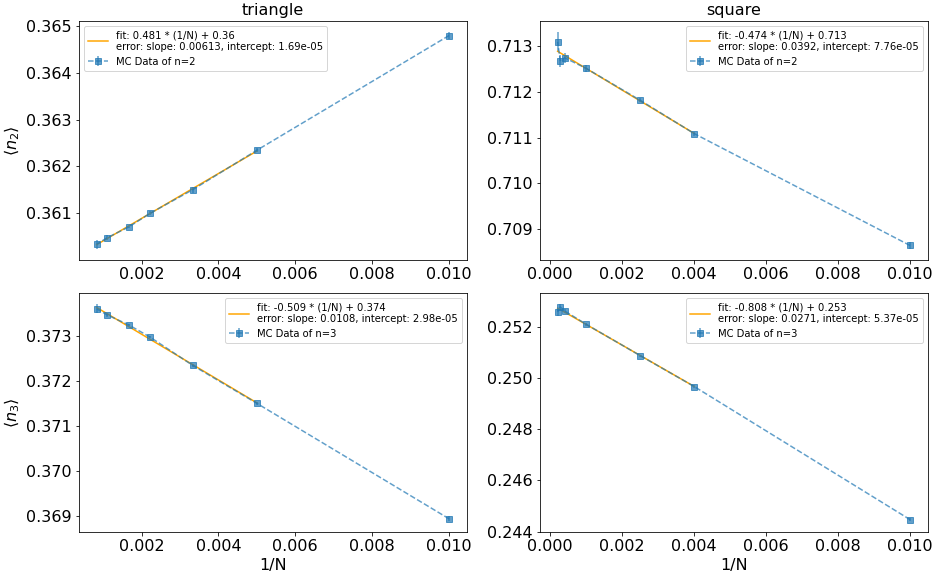
\includegraphics[width=0.95\textwidth]{Sections/Images/triagle_vs_square_bulk.png}
    \caption{Графики зависимости средней доли узлов с 2-3-мя соседями (сверху вниз) от обратной длины 1/N в модели Изинга на треугольной (слева) и квадратной (справа) решётках при J=0. Синяя линия описывает результаты симуляций Монте-Карло, оранжевая - линейное приближение на всех точках кроме первой}
    \label{fig:tr_vs_sq_bulk}
\end{figure}

На графике \ref{fig:tr_vs_sq_bulk} наглядно показано сравнение приближений долей одномерий и узлов с тремя соседями в цепочках на треугольной и квадратной решётках. Для расчётов долей на треугольной решётке были использованы длины 100-1200, для квадратной - 100-4900. Приближение долей треугольной решётки имеет отчётливый линейный характер, включая даже в приближении на всех точках (см. раздел "Подсчёт соседей у треугольной решётки" в Bulk2-6.ipynb\cite{Git}). Линейность долей квадратной решётки также подтверждается (с учётом погрешности расчётов с наибольшей длинной, возможно требуются расчёты дольше 2-х дней).

Так же хочется заметить некоторое сходство значений свободного члена для долей с двумя соседями и свободного члена в приближениях графика зависимости вероятности гомополимерной цепочки иметь атмосферу 3 в статье Преллберга\cite{Prellberg} (то есть вероятность, что второй конец цепочки длины N имеет 3 возможных направления для удлинения и следовательно, 3 узла, которые могут стать N+1-ым в цепочке), хотя сами приближения имеют противоположные по знаку наклоны. Возможно, обе величины по-разному описывают одно и то же одномерное поведение цепочек.

Однако сходства между одномерием треугольной и квадратной решётки с точки зрения самих приближений почти не наблюдается - они имеют как разные значения свободных членов, так и коэф. наклона, разница значительно превышает погрешность фита. 

\subsection{Сравнение геометрических свойств модели Изинга на треугольной решётке с кубической}

\begin{figure}
    \centering
    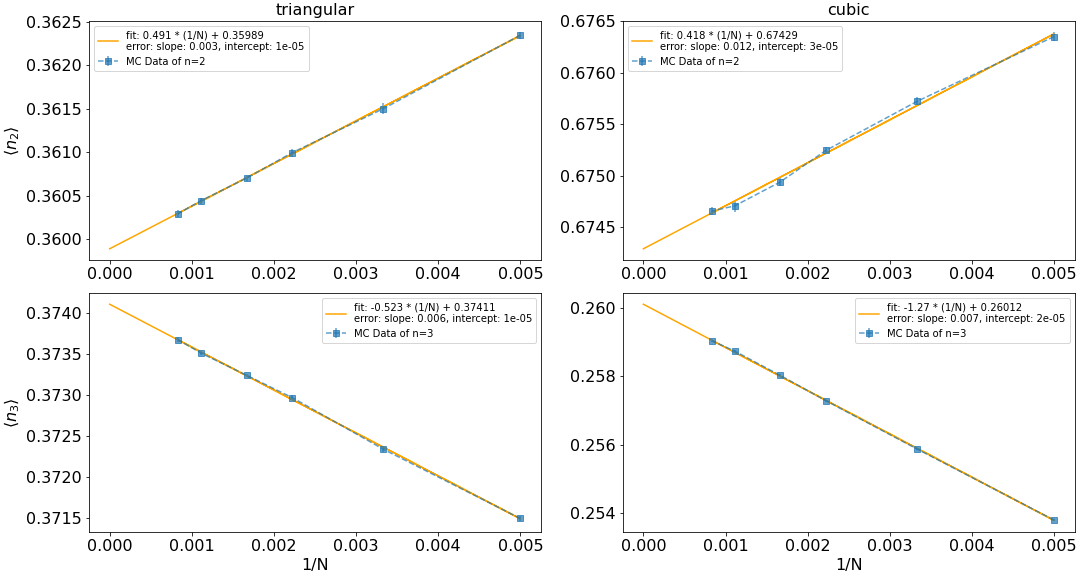
\includegraphics[width=0.95\textwidth]{Sections/Images/triangle_vs_cubic_bulk.png}
    \caption{Графики зависимости средней доли узлов с 2-3-мя соседями (сверху вниз) от обратной длины 1/N в модели Изинга на треугольной (слева) и кубической (справа) решётках при J=0. Синяя линия описывает результаты симуляций Монте-Карло, оранжевая - линейное приближение на всех точках кроме первой}
    \label{fig:tr_vs_cb_bulk}
\end{figure}

Здесь примерно та же ситуация - кубическая решётка на графике \ref{fig:tr_vs_cb_bulk} показывает почти чёткий линейный характер приближения в пределах погрешности наибольших длин (для n=3 линейно видна значительно лучше), но значения не имеют никакого сходства. Единственное отличие от сравнения с квадратной решёткой - графики соответствующих долей имеют одинаковое поведение с точки зрения знака наклона, что действительно и для долей узлов с больший числом соседей